% ChessReasoner-120M architecture figure.
% Standalone: compile with `tectonic chessreasoner_arch.tex` -> chessreasoner_arch.pdf
% In the paper:  
\includegraphics[width=\textwidth]{figures/chessreasoner_arch.pdf}
\documentclass[border=6pt]{standalone}
\usepackage{tikz}
\usepackage{amsmath}
\usepackage[T1]{fontenc}
\usepackage{newtxtext,newtxmath}
\usetikzlibrary{arrows.meta,positioning,fit,backgrounds,calc,decorations.pathreplacing}

\definecolor{navy}{RGB}{27,64,105}
\definecolor{teal}{RGB}{18,112,122}
\definecolor{amber}{RGB}{171,110,18}
\definecolor{slate}{RGB}{92,102,114}
\definecolor{paleblue}{RGB}{226,236,246}
\definecolor{paleteal}{RGB}{221,239,239}
\definecolor{paleamber}{RGB}{251,241,224}
\definecolor{paleslate}{RGB}{239,241,244}
\definecolor{rulegray}{RGB}{168,176,187}

\begin{document}
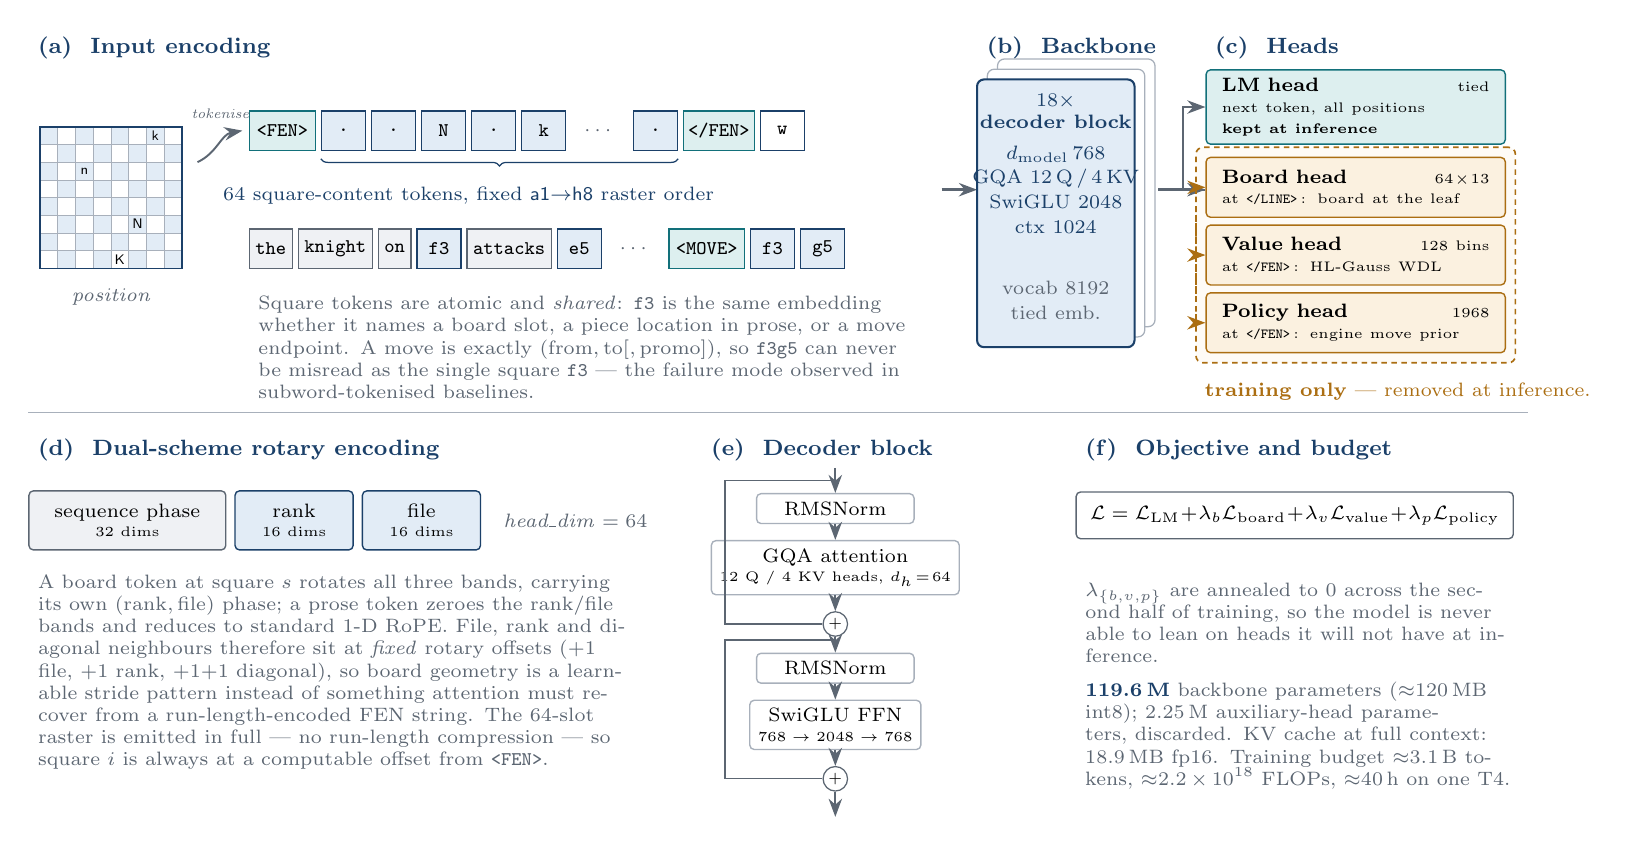
\begin{tikzpicture}[
  font=\small,
  >={Stealth[length=2.3mm,width=1.7mm]},
  box/.style={rounded corners=1.6pt,draw=rulegray,line width=0.5pt,align=center,inner sep=3pt},
  tok/.style={draw=navy,fill=paleblue,line width=0.45pt,minimum width=5.6mm,minimum height=5.0mm,
              inner sep=0pt,font=\scriptsize},
  mtok/.style={tok,draw=teal,fill=paleteal},
  word/.style={draw=slate,fill=paleslate,line width=0.45pt,minimum height=5.0mm,
               inner sep=2.2pt,font=\scriptsize},
  head/.style={box,fill=white,minimum width=38mm,minimum height=7.6mm,font=\scriptsize,align=left,
               text width=34mm},
  aux/.style={head,draw=amber,fill=paleamber},
  lmh/.style={head,draw=teal,fill=paleteal},
  lbl/.style={font=\scriptsize\itshape,text=slate},
  sec/.style={font=\bfseries\footnotesize,text=navy},
  note/.style={font=\scriptsize,text=slate,align=left},
  flow/.style={->,draw=slate,line width=0.7pt},
  tap/.style={->,draw=amber,line width=0.65pt,dashed,dash pattern=on 1.6pt off 1.4pt},
  panel/.style={rounded corners=2.5pt,draw=rulegray,line width=0.45pt,fill=white},
]

% =====================================================================
% ============================ TOP: PIPELINE ==========================
% =====================================================================

\node[sec,anchor=west] at (0.0,10.35) {(a)\ \ Input encoding};
\node[sec,anchor=west] at (12.05,10.35) {(b)\ \ Backbone};
\node[sec,anchor=west] at (14.95,10.35) {(c)\ \ Heads};

% ---------------- chess board ----------------
\begin{scope}[shift={(0.15,7.55)},scale=0.225]
  \foreach \r in {0,...,7}{\foreach \f in {0,...,7}{
    \pgfmathparse{mod(\r+\f,2)==0 ? "white" : "paleblue"}
    \edef\cc{\pgfmathresult}
    \draw[fill=\cc,draw=rulegray,line width=0.2pt] (\f,\r) rectangle ++(1,1);}}
  \node[font=\tiny] at (6.5,7.5) {\textsf{k}};
  \node[font=\tiny] at (2.5,5.5) {\textsf{n}};
  \node[font=\tiny] at (5.5,2.5) {\textsf{N}};
  \node[font=\tiny] at (4.5,0.5) {\textsf{K}};
  \draw[draw=navy,line width=0.6pt] (0,0) rectangle (8,8);
\end{scope}
\node[lbl,anchor=north] at (1.05,7.42) {position};

\draw[flow] (2.15,8.90) to[out=25,in=190] (2.72,9.30);
\node[lbl,anchor=south,font=\tiny\itshape] at (2.44,9.33) {tokenise};

% ---------------- token row 1: board plane ----------------
\node[mtok,anchor=west,minimum width=8.4mm] (bfen) at (2.80,9.30) {\texttt{<FEN>}};
\node[tok,right=0.6mm of bfen] (p1) {\texttt{.}};
\node[tok,right=0.6mm of p1]   (p2) {\texttt{.}};
\node[tok,right=0.6mm of p2]   (p3) {\texttt{N}};
\node[tok,right=0.6mm of p3]   (p4) {\texttt{.}};
\node[tok,right=0.6mm of p4]   (p5) {\texttt{k}};
\node[right=1.0mm of p5,font=\scriptsize,text=slate] (pd) {$\cdots$};
\node[tok,right=1.0mm of pd]   (p6) {\texttt{.}};
\node[mtok,right=0.6mm of p6,minimum width=9.0mm] (efen) {\texttt{</FEN>}};
\node[tok,right=0.6mm of efen,fill=white] (stm) {\texttt{w}};

\draw[decorate,decoration={brace,amplitude=2.6pt,mirror},draw=navy,line width=0.45pt]
  ($(p1.south west)+(0,-1.0mm)$) -- ($(p6.south east)+(0,-1.0mm)$);
\node[font=\scriptsize,text=navy,anchor=north] at ($(p3.south)!0.5!(p4.south)+(0,-3.4mm)$)
  {64 square-content tokens, fixed \textsf{a1}$\rightarrow$\textsf{h8} raster order};

% ---------------- token row 2: prose + move ----------------
\node[word,anchor=west] (w1) at (2.80,7.80) {\texttt{the}};
\node[word,right=0.6mm of w1] (w2) {\texttt{knight}};
\node[word,right=0.6mm of w2] (w3) {\texttt{on}};
\node[tok,right=0.6mm of w3]  (w4) {\texttt{f3}};
\node[word,right=0.6mm of w4] (w5) {\texttt{attacks}};
\node[tok,right=0.6mm of w5]  (w6) {\texttt{e5}};
\node[right=1.0mm of w6,font=\scriptsize,text=slate] (wd) {$\cdots$};
\node[mtok,right=1.0mm of wd,minimum width=9.6mm] (mv) {\texttt{<MOVE>}};
\node[tok,right=0.6mm of mv] (mf) {\texttt{f3}};
\node[tok,right=0.6mm of mf] (mt) {\texttt{g5}};

\node[note,anchor=north west,text width=88mm] at (2.80,7.32)
  {Square tokens are atomic and \emph{shared}: \texttt{f3} is the same embedding whether it
   names a board slot, a piece location in prose, or a move endpoint. A move is exactly
   $(\text{from},\text{to}[,\text{promo}])$, so \texttt{f3g5} can never be misread as the
   single square \texttt{f3} --- the failure mode observed in subword-tokenised baselines.};

% ---------------- backbone ----------------
\draw[flow,line width=0.9pt] (11.60,8.55) -- (12.05,8.55);

\begin{scope}
  \foreach \dx/\dy in {0.26/0.26, 0.13/0.13}{
    \draw[rounded corners=2.5pt,draw=rulegray,fill=white,line width=0.45pt]
      (12.05+\dx,6.55+\dy) rectangle (14.05+\dx,9.95+\dy);}
  \draw[rounded corners=2.5pt,draw=navy,fill=paleblue,line width=0.75pt]
    (12.05,6.55) rectangle (14.05,9.95);
\end{scope}
\node[font=\bfseries\scriptsize,text=navy,align=center] at (13.05,9.55) {$18\times$\\ decoder block};
\node[font=\scriptsize,text=navy,align=center] at (13.05,8.55)
  {$d_{\text{model}}$\,768\\[1pt] GQA 12\,Q\,/\,4\,KV\\[1pt] SwiGLU 2048\\[1pt] ctx 1024};
\node[font=\scriptsize,text=slate,align=center] at (13.05,7.15) {vocab 8192\\[1pt] tied emb.};

\draw[flow,line width=0.9pt] (14.35,8.55) -- (14.95,8.55);

% ---------------- heads ----------------
\node[lmh,anchor=west]  (hlm)    at (14.95,9.60)
  {\textbf{LM head}\hfill{\tiny tied}\\[-0.5pt]{\tiny next token, all positions}\\[-0.5pt]{\tiny \textbf{kept at inference}}};
\node[aux,anchor=west]  (hboard) at (14.95,8.58)
  {\textbf{Board head}\hfill{\tiny $64\!\times\!13$}\\[-0.5pt]{\tiny at \texttt{</LINE>}\,: board at the leaf}};
\node[aux,anchor=west]  (hval)   at (14.95,7.72)
  {\textbf{Value head}\hfill{\tiny 128 bins}\\[-0.5pt]{\tiny at \texttt{</FEN>}\,: HL-Gauss WDL}};
\node[aux,anchor=west]  (hpol)   at (14.95,6.86)
  {\textbf{Policy head}\hfill{\tiny 1968}\\[-0.5pt]{\tiny at \texttt{</FEN>}\,: engine move prior}};

\draw[flow] (14.95,8.55) -- ++(-0.28,0) |- (hlm.west);
\draw[tap]  (14.83,8.55) |- (hboard.west);
\draw[tap]  (14.83,8.55) |- (hval.west);
\draw[tap]  (14.83,8.55) |- (hpol.west);

\begin{scope}[on background layer]
  \node[draw=amber,dashed,dash pattern=on 2pt off 1.6pt,rounded corners=2.5pt,line width=0.6pt,
        fill=paleamber!30,fit=(hboard)(hval)(hpol),inner sep=3.4pt] (auxbox) {};
\end{scope}

\node[font=\scriptsize,text=amber,anchor=north west,align=left] at ($(auxbox.south west)+(0,-1.2mm)$)
  {\textbf{training only} --- removed at inference.};

% =====================================================================
% ========================= BOTTOM: DETAIL PANELS =====================
% =====================================================================

\draw[draw=rulegray,line width=0.4pt] (0,5.72) -- (19.05,5.72);

% ---------------- (d) dual-scheme RoPE ----------------
\node[sec,anchor=west] at (0.0,5.25) {(d)\ \ Dual-scheme rotary encoding};

\node[box,fill=paleslate,draw=slate,minimum width=25mm,minimum height=7.5mm,anchor=west,font=\scriptsize]
  (bseq) at (0.0,4.35) {sequence phase\\[-1pt]{\tiny 32 dims}};
\node[box,fill=paleblue,draw=navy,minimum width=15mm,minimum height=7.5mm,right=1.0mm of bseq,font=\scriptsize]
  (brank) {rank\\[-1pt]{\tiny 16 dims}};
\node[box,fill=paleblue,draw=navy,minimum width=15mm,minimum height=7.5mm,right=1.0mm of brank,font=\scriptsize]
  (bfile) {file\\[-1pt]{\tiny 16 dims}};
\node[lbl,anchor=west] at ($(bfile.east)+(1.6mm,0)$) {head\_dim $=64$};

\node[note,anchor=north west,text width=76mm] at (0.0,3.78)
  {A board token at square $s$ rotates all three bands, carrying its own
   $(\text{rank},\text{file})$ phase; a prose token zeroes the rank/file bands and
   reduces to standard 1-D RoPE. File, rank and diagonal neighbours therefore sit at
   \emph{fixed} rotary offsets ($+1$ file, $+1$ rank, $+1{+}1$ diagonal), so board
   geometry is a learnable stride pattern instead of something attention must recover
   from a run-length-encoded FEN string. The 64-slot raster is emitted in full --- no
   run-length compression --- so square $i$ is always at a computable offset from
   \texttt{<FEN>}.};

% ---------------- (e) block detail ----------------
\node[sec,anchor=west] at (8.55,5.25) {(e)\ \ Decoder block};

\begin{scope}[shift={(9.30,0.0)}]
  \node[box,fill=white,minimum width=20mm,font=\scriptsize] (rms1) at (0.95,4.50) {RMSNorm};
  \node[box,fill=white,minimum width=20mm,font=\scriptsize,below=2.0mm of rms1] (att)
    {GQA attention\\[-1pt]{\tiny 12 Q / 4 KV heads, $d_h\!=\!64$}};
  \node[circle,draw=slate,line width=0.45pt,inner sep=0.8pt,font=\tiny,below=2.0mm of att] (add1) {$+$};
  \node[box,fill=white,minimum width=20mm,font=\scriptsize,below=2.0mm of add1] (rms2) {RMSNorm};
  \node[box,fill=white,minimum width=20mm,font=\scriptsize,below=2.0mm of rms2] (ffn)
    {SwiGLU FFN\\[-1pt]{\tiny $768\rightarrow2048\rightarrow768$}};
  \node[circle,draw=slate,line width=0.45pt,inner sep=0.8pt,font=\tiny,below=2.0mm of ffn] (add2) {$+$};

  \draw[flow] (rms1) -- (att);   \draw[flow] (att) -- (add1);
  \draw[flow] (add1) -- (rms2);  \draw[flow] (rms2) -- (ffn);
  \draw[flow] (ffn) -- (add2);
  \draw[draw=slate,line width=0.45pt] ($(rms1.north)+(0,1.6mm)$) -- ++(-14mm,0) |- (add1.west);
  \draw[draw=slate,line width=0.45pt] ($(rms2.north)+(0,1.6mm)$) -- ++(-14mm,0) |- (add2.west);
  \draw[flow] ($(rms1.north)+(0,3.2mm)$) -- (rms1.north);
  \draw[flow] (add2.south) -- ++(0,-3.2mm);
\end{scope}

% ---------------- (f) objective + budget ----------------
\node[sec,anchor=west] at (13.30,5.25) {(f)\ \ Objective and budget};

\node[box,fill=white,draw=slate,anchor=north west,font=\scriptsize,align=left,inner sep=5pt,
      text width=52mm] (loss) at (13.30,4.72)
  {$\mathcal{L}=\mathcal{L}_{\text{LM}}
      +\lambda_{b}\mathcal{L}_{\text{board}}
      +\lambda_{v}\mathcal{L}_{\text{value}}
      +\lambda_{p}\mathcal{L}_{\text{policy}}$};

\node[note,anchor=north west,text width=54mm] at (13.30,3.68)
  {$\lambda_{\{b,v,p\}}$ are annealed to $0$ across the second half of training, so the
   model is never able to lean on heads it will not have at inference.};

\node[note,anchor=north west,text width=54mm] at (13.30,2.42)
  {\textbf{\textcolor{navy}{119.6\,M}} backbone parameters ($\approx$120\,MB int8);
   $2.25$\,M auxiliary-head parameters, discarded.
   KV cache at full context: $18.9$\,MB fp16.
   Training budget $\approx$$3.1$\,B tokens,
   $\approx$$2.2\times10^{18}$ FLOPs, $\approx$40\,h on one T4.};

\end{tikzpicture}
\end{document}
